\section{The spherical coordinate system}
\label{Sec1:sphericalCoordinates}
The spherical coordinate system is defined by the transformation $\vec{x}(r,\vartheta,\varphi)=x_i(r,\vartheta,\varphi)\vec{e}_i$, where $\vec{e}_i$ are the standard basis vectors in the Cartesian coordinate system and (see \Cref{Fig1:SphericalCoordinateSystem})
\begin{figure}
	\centering
	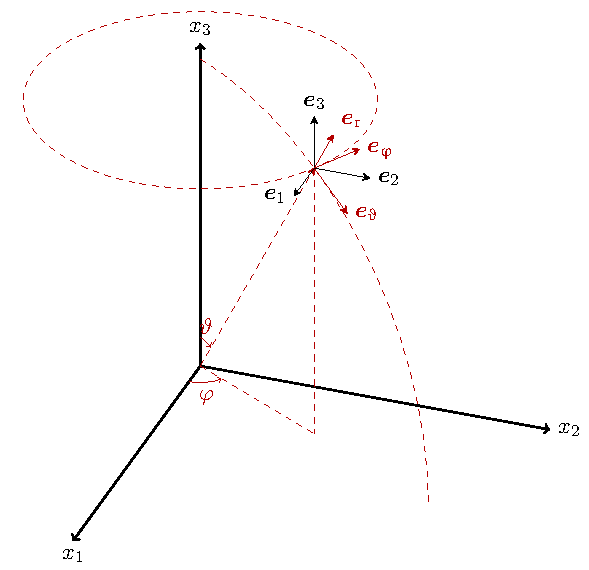
\includegraphics{sphericalCoordinateSystem}
	\caption{The spherical and Cartesian coordinate system.}
	\label{Fig1:SphericalCoordinateSystem}
\end{figure}
\begin{align}
	x_1 &= r\sin\vartheta\cos\varphi\\
	x_2 &= r\sin\vartheta\sin\varphi\\
	x_3 &= r\cos\vartheta.
\end{align}
The inverse relation is then found to be
\begin{align}
	r &= |\vec{x}|,\quad\text{with}\quad |\vec{x}|=\sqrt{x_1^2+x_2^2+x_3^2}\\
	\vartheta &= \arccos\left(\frac{x_3}{|\vec{x}|}\right)\\
	\varphi &= \operatorname{atan2}(x_2,x_1),
\end{align}
where
\begin{equation}
	\operatorname{atan2}(x_2,x_1) = \begin{cases}
	\arctan(\frac{x_2}{x_1}) & \mbox{if } x_1 > 0\\
	\arctan(\frac{x_2}{x_1}) + \PI & \mbox{if } x_1 < 0 \mbox{ and } x_2 \ge 0\\
	\arctan(\frac{x_2}{x_1}) - \PI & \mbox{if } x_1 < 0 \mbox{ and } x_2 < 0\\
	\frac{\PI}{2} & \mbox{if } x_1 = 0 \mbox{ and } x_2 > 0\\
	-\frac{\PI}{2} & \mbox{if } x_1 = 0 \mbox{ and } x_2 < 0\\
	\text{undefined} & \mbox{if } x_1 = 0 \mbox{ and } x_2 = 0.
	\end{cases}
\end{equation}
Hence, the Jacobian matrix of the spherical transformation is given by
\begin{equation}
	\vec{J}_{\mathrm{s}} = \begin{bmatrix}
		\pderiv{x_1}{r} & \pderiv{x_1}{\vartheta} & \pderiv{x_1}{\varphi}\\
		\pderiv{x_2}{r} & \pderiv{x_2}{\vartheta} & \pderiv{x_2}{\varphi}\\
		\pderiv{x_3}{r} & \pderiv{x_3}{\vartheta} & \pderiv{x_3}{\varphi}
	\end{bmatrix} = \begin{bmatrix}
		\sin\vartheta\cos\varphi & r\cos\vartheta\cos\varphi & -r\sin\vartheta\sin\varphi\\
		\sin\vartheta\sin\varphi & r\cos\vartheta\sin\varphi & r\sin\vartheta\cos\varphi\\
		\cos\vartheta & -r\sin\vartheta & 0
	\end{bmatrix}
\end{equation}
with inverse given by
\begin{equation}
	\vec{J}_{\mathrm{s}}^{-1} = \begin{bmatrix}
		\pderiv{r}{x_1} & \pderiv{r}{x_2} & \pderiv{r}{x_3}\\
		\pderiv{\vartheta}{x_1} & \pderiv{\vartheta}{x_2} & \pderiv{\vartheta}{x_3}\\
		\pderiv{\varphi}{x_1} & \pderiv{\varphi}{x_2} & \pderiv{\varphi}{x_3}
	\end{bmatrix} = \begin{bmatrix}
		\sin\vartheta\cos\varphi & \sin\vartheta\sin\varphi & \cos\vartheta\\
		\frac{1}{r}\cos\vartheta\cos\varphi & \frac{1}{r}\cos\vartheta\sin\varphi & -\frac{1}{r}\sin\vartheta\\
		-\frac{1}{r}\frac{\sin\varphi}{\sin\vartheta} & \frac{1}{r}\frac{\cos\varphi}{\sin\vartheta} & 0
	\end{bmatrix}.
\end{equation}
So for a scalar valued function $\Psi$ the following is obtained (using the chain rule)
\begin{equation}
\label{Eq1:derivativesInSphericalCoordinates}
	\begin{bmatrix}
		\pderiv{\Psi}{r}\\
		\pderiv{\Psi}{\vartheta}\\
		\pderiv{\Psi}{\varphi}
	\end{bmatrix} = \vec{J}_{\mathrm{s}}^{\transpose} 
	\begin{bmatrix}
		\pderiv{\Psi}{x_1}\\
		\pderiv{\Psi}{x_2}\\
		\pderiv{\Psi}{x_3}
	\end{bmatrix}.
\end{equation}
The scale factors in the spherical coordinate system are given by
\begin{equation}
	h_{\mathrm{r}} = \left|\pderiv{\vec{x}}{r}\right| = 1,\quad h_\upvartheta = \left|\pderiv{\vec{x}}{\vartheta}\right| = r,\quad h_\upvarphi = \left|\pderiv{\vec{x}}{\varphi}\right| = r\sin\theta,
\end{equation}
from which the following basis vectors are derived (see \Cref{Fig1:SphericalCoordinateSystem})
\begin{align}
	\vec{e}_{\mathrm{r}} &= \frac{1}{h_{\mathrm{r}}}\pderiv{\vec{x}}{r} = \vec{e}_1\sin\vartheta\cos\varphi + \vec{e}_2\sin\vartheta\sin\varphi + \vec{e}_3\cos\vartheta\\
	\vec{e}_{\upvartheta} &= \frac{1}{h_\upvartheta}\pderiv{\vec{x}}{\vartheta} = \vec{e}_1\cos\vartheta\cos\varphi + \vec{e}_2\cos\vartheta\sin\varphi - \vec{e}_3\sin\vartheta\\
	\vec{e}_{\upvarphi} &= \frac{1}{h_\upvarphi}\pderiv{\vec{x}}{\varphi} = -\vec{e}_1\sin\varphi + \vec{e}_2\cos\varphi.
\end{align}
This can be written in the following matrix form
\begin{equation}
\label{Eq1:XtoSpherical}
	\begin{bmatrix}
		\vec{e}_{\mathrm{r}} & \vec{e}_{\upvartheta} & \vec{e}_{\upvarphi}
	\end{bmatrix} = \vec{J}_{\mathrm{e}}^\transpose\begin{bmatrix}
		\vec{e}_1 & \vec{e}_2 & \vec{e}_3
	\end{bmatrix} = \vec{J}_{\mathrm{e}}^\transpose
\end{equation}
where
\begin{equation}
	\vec{J}_{\mathrm{e}} = \begin{bmatrix}
		\sin\vartheta\cos\varphi & \sin\vartheta\sin\varphi & \cos\vartheta\\
		\cos\vartheta\cos\varphi & \cos\vartheta\sin\varphi & -\sin\vartheta\\
		-\sin\varphi & \cos\varphi & 0
	\end{bmatrix}
\end{equation}
and inverse given by
\begin{equation}
	\vec{J}_{\mathrm{e}}^{-1} = \begin{bmatrix}
		\sin\vartheta\cos\varphi & \cos\vartheta\cos\varphi & -\sin\varphi\\
		\sin\vartheta\sin\varphi & \cos\vartheta\sin\varphi & \cos\varphi\\
		\cos\vartheta & -\sin\vartheta & 0
	\end{bmatrix}.
\end{equation}
So, for any vector field
\begin{equation}
	\vec{\Psi} = \Psi_1\vec{e}_1 + \Psi_2\vec{e}_2  + \Psi_3\vec{e}_3 = \Psi_{\mathrm{r}}\vec{e}_{\mathrm{r}} + \Psi_{\upvartheta}\vec{e}_{\upvartheta} + \Psi_{\upvarphi}\vec{e}_{\upvarphi} 
\end{equation}
the following relation is found (by comparing each component)
\begin{equation}
\label{Eq1:SphericalToXfun}
	\begin{bmatrix}
		\Psi_1\\
		\Psi_2\\
		\Psi_3
	\end{bmatrix} = \vec{J}_{\mathrm{e}}^{\transpose} 
	\begin{bmatrix}
		\Psi_{\mathrm{r}}\\
		\Psi_{\upvartheta}\\
		\Psi_{\upvarphi}
	\end{bmatrix},
\end{equation}
and the Jacobian of $\vec{\Psi}$ is given by (using the chain rule)
\begin{align}
\label{Eq1:SphericalToXJacobian}
\begin{split}
	\begin{bmatrix}
		\pderiv{\Psi_1}{x_1} & \pderiv{\Psi_1}{x_2} & \pderiv{\Psi_1}{x_3}\\
		\pderiv{\Psi_2}{x_1} & \pderiv{\Psi_2}{x_2} & \pderiv{\Psi_2}{x_3}\\
		\pderiv{\Psi_3}{x_1} & \pderiv{\Psi_3}{x_2} & \pderiv{\Psi_3}{x_3}
	\end{bmatrix} &= \begin{bmatrix}
		\pderiv{\Psi_1}{r} & \pderiv{\Psi_1}{\vartheta} & \pderiv{\Psi_1}{\varphi}\\
		\pderiv{\Psi_2}{r} & \pderiv{\Psi_2}{\vartheta} & \pderiv{\Psi_2}{\varphi}\\
		\pderiv{\Psi_3}{r} & \pderiv{\Psi_3}{\vartheta} & \pderiv{\Psi_3}{\varphi}
	\end{bmatrix}\vec{J}_{\mathrm{s}}^{-1} \\
	&= \left(\vec{J}_1\Psi_{\mathrm{r}}+\vec{J}_2\Psi_{\upvartheta}+\vec{J}_3\Psi_{\upvarphi} + \vec{J}_{\mathrm{e}}^{\transpose}\begin{bmatrix}
		\pderiv{\Psi_{\mathrm{r}}}{r} & \pderiv{\Psi_{\mathrm{r}}}{\vartheta} & \pderiv{\Psi_{\mathrm{r}}}{\varphi}\\
		\pderiv{\Psi_{\upvartheta}}{r} & \pderiv{\Psi_{\upvartheta}}{\vartheta} & \pderiv{\Psi_{\upvartheta}}{\varphi}\\
		\pderiv{\Psi_{\upvarphi}}{r} & \pderiv{\Psi_{\upvarphi}}{\vartheta} & \pderiv{\Psi_{\upvarphi}}{\varphi}
	\end{bmatrix}\right)\vec{J}_{\mathrm{s}}^{-1}
	\end{split}
\end{align}
where
\begin{align*}
	&\vec{J}_1 = \begin{bmatrix}
		0 & \cos\vartheta\cos\varphi & -\sin\vartheta\sin\varphi\\
		0 & \cos\vartheta\sin\varphi & \sin\vartheta\cos\varphi\\
		0 & -\sin\vartheta & 0
	\end{bmatrix},\quad\vec{J}_2 = \begin{bmatrix}
		0 & -\sin\vartheta\cos\varphi & -\cos\vartheta\sin\varphi\\
		0 & -\sin\vartheta\sin\varphi & \cos\vartheta\cos\varphi\\
		0 & -\cos\vartheta & 0
	\end{bmatrix},\\
	&\vec{J}_3 = \begin{bmatrix}
		0 & 0 & -\cos\varphi\\
		0 & 0 & -\sin\varphi\\
		0 & 0 & 0
	\end{bmatrix}.
\end{align*}
Using \Cref{Eq1:derivativesInSphericalCoordinates,Eq1:SphericalToXfun,Eq1:XtoSpherical}, the following formulas are obtained
\begin{align}
	\nabla\Psi &= \pderiv{\Psi}{r}\vec{e}_{\mathrm{r}}+\frac{1}{r}\pderiv{\Psi}{\vartheta}\vec{e}_{\upvartheta}+\frac{1}{r\sin\vartheta}\pderiv{\Psi}{\varphi}\vec{e}_{\upvarphi} \label{Eq1:delScalarSpherical} \\	
	\nabla^2\Psi &= \frac{1}{r^2}\pderiv{}{r}\left(r^2\pderiv{\Psi}{r}\right) + \frac{1}{r^2\sin\vartheta}\pderiv{}{\vartheta}\left(\sin\vartheta\pderiv{\Psi}{\vartheta}\right) +\frac{1}{r^2\sin^2\vartheta}\pderiv[2]{\Psi}{\varphi} \label{Eq1:laplaceScalarSpherical}\\
	\nabla\cdot\vec{\Psi} &= \frac{1}{r^2}\pderiv{(r^2\Psi_{\mathrm{r}})}{r} + \frac{1}{r\sin\vartheta}\pderiv{(\Psi_{\upvartheta}\sin\vartheta)}{\vartheta}+\frac{1}{r\sin\vartheta}\pderiv{\Psi_{\upvarphi}}{\varphi} \label{Eq1:DelDotVecSpherical} \\ 
	\begin{split}\nabla^2\vec{\Psi} &= \left(\nabla^2\Psi_{\mathrm{r}} - \frac{2}{r^2}\Psi_{\mathrm{r}}-\frac{2}{r^2\sin\vartheta}\pderiv{(\Psi_{\upvartheta}\sin\vartheta)}{\vartheta} -\frac{2}{r^2\sin\vartheta}\pderiv{\Psi_{\upvarphi}}{\varphi}\right)\vec{e}_{\mathrm{r}} \\
	&{\hskip1em\relax}+ \left(\nabla^2\Psi_{\upvartheta}-\frac{1}{r^2\sin^2\vartheta}\Psi_{\upvartheta} + \frac{2}{r^2}\pderiv{\Psi_{\mathrm{r}}}{\vartheta} -\frac{2\cos\vartheta}{r^2\sin^2\vartheta}\pderiv{\Psi_{\upvarphi}}{\varphi}\right)\vec{e}_{\upvartheta} \\
	&{\hskip1em\relax}+ \left(\nabla^2\Psi_{\upvarphi} - \frac{1}{r^2\sin^2\vartheta}\Psi_{\upvarphi} + \frac{2}{r^2\sin\vartheta}\pderiv{\Psi_{\mathrm{r}}}{\varphi}+\frac{2\cos\vartheta}{r^2\sin^2\vartheta}\pderiv{\Psi_{\upvartheta}}{\varphi}\right)\vec{e}_{\upvarphi} \end{split}\label{Eq1:LapVecPotSpherical}\\
	\begin{split}
	\nabla\times\vec{\Psi} &=  \frac{1}{r\sin\vartheta}\left(\pderiv{}{\vartheta}\left(\Psi_\upvarphi\sin\vartheta\right) - \pderiv{\Psi_\upvartheta}{\varphi}\right)\vec{e}_{\mathrm{r}} + \frac{1}{r}\left(\frac{1}{\sin\vartheta}\pderiv{\Psi_{\mathrm{r}}}{\varphi} - \pderiv{}{r}\left(r\Psi_\upvarphi\right)\right)\vec{e}_\upvartheta\\
	&{\hskip1em\relax}+ \frac{1}{r}\left(\pderiv{}{r}\left(r\Psi_\upvartheta\right) - \pderiv{\Psi_{\mathrm{r}}}{\vartheta}\right)\vec{e}_\upvarphi.
	\end{split}\label{Eq1:CrossVecPotSpherical}
\end{align}
